\section{Topology Skeletons}
Even though many algorithms can be expressed by parallel maps, some problems require more sophisticated skeletons. The Eden library leverages this problem and already comes with more predefined skeletons, among them are a \code{pipe}, \code{ring} and a \code{torus} implementation \cite{eden_cefp, eden_skel_topology}. These seem like reasonable candidates to be ported to our arrow based parallel Haskell to prove that we can express such skeletons with Arrows as well.

\subsection{pipe}

The parallel pipe skeleton is semantically equivalent to folding over a list \code{[arr a a]} of arrows with \code{>>>}, but does this in parallel, meaning that the arrows don't have to reside on the same thread/machine. We implement this skeleton using the \code{ArrowLoop} typeclass which enables us to use \code{loop :: arr (a, b) (c, b) -> arr a c}.

\begin{lstlisting}[frame=htrbl]
pipeSimple :: (ArrowLoop arr, ArrowParallel arr a a conf) =>
	conf -> [arr a a] -> arr a a
pipeSimple conf fs =
	loop (arr snd &&& (arr (uncurry (:) >>> lazy) >>>
		parEvalN conf fs)) >>>
	arr last
\end{lstlisting}
where \code{lazy} is defined as:
\begin{lstlisting}[frame=htrbl]
lazy :: (Arrow arr) => arr [a] [a]
lazy = arr (\ ~(x:xs) -> x : lazy xs)
\end{lstlisting}
However, using this definition directly, will result in the master node becoming a potential bottleneck in distributed environments as described in chapter \ref{futures}. Therefore, a more sophisticated version that uses Futures internally is a good idea:
\begin{lstlisting}[frame=htrbl]
pipe :: (ArrowLoop arr, ArrowParallel arr (fut a) (fut a) conf,
	Future fut a) =>
	conf -> [arr a a] -> arr a a
pipe conf fs = unliftFut (pipeSimple conf (map liftFut fs))
\end{lstlisting}
Sometimes, this pipe definition can be a bit inconvenient, especially if we want to pipe arrows of mixed types together, i.e. \code{arr a b} and \code{arr b c}. By wrapping these two arrows inside a common type
\begin{lstlisting}[frame=htrbl]
pipe2 :: (ArrowLoop arr, ArrowChoice arr,
	ArrowParallel arr (fut (([a], [b]), [c])) (fut (([a], [b]), [c])) conf,
	Future fut (([a], [b]), [c])) =>
	conf -> arr a b -> arr b c -> arr a c
pipe2 conf f g = 
	(arr return &&& arr (const [])) &&& arr (const []) >>>
	pipe conf (replicate 2 (unify f g)) >>>
	arr snd >>>
	arr head
		where
			unify :: (ArrowChoice arr) =>
				arr a b -> arr b c -> arr (([a], [b]), [c]) (([a], [b]), [c])
			unify f g =
				(mapArr f *** mapArr g) *** arr (\_ -> []) >>>
				arr (\((a, b), c) -> ((c, a), b))
\end{lstlisting}
Note that extensive use of this combinator over \code{pipe} with a hand-written combination data-type will probably result in worse performance because of more communication overhead from the many calls to parEvalN. Nonetheless, we can define a parallel piping operator \code{|>>>|} which is semantically equivalent to \code{>>>} similar to the other parallel syntactic sugar from chapter \ref{syntacticSugar}:
\begin{lstlisting}[frame=htrbl]
(|>>>|) :: (ArrowLoop arr, ArrowChoice arr,
	ArrowParallel arr (fut (([a], [b]), [c])) (fut (([a], [b]), [c])) (),
	Future fut (([a], [b]), [c])) =>
	arr a b -> arr b c -> arr a c
(|>>>|) = pipe2 ()
\end{lstlisting}

\subsection{ring}
\begin{center}
	\includegraphics[scale=0.75]{images/ring}
\end{center}
\begin{lstlisting}[frame=htrbl]
ring :: (ArrowLoop arr, Future fut r,
	ArrowParallel arr (i, fut r) (o, fut r) conf) =>
    conf ->
    arr (i, r) (o, r) ->
    arr [i] [o]
ring conf f =
	loop (second (rightRotate >>> lazy) >>>
    arr (uncurry zip) >>>
    parMap conf (second get >>> f >>> second put) >>>
    arr unzip)

-- from Eden, ported to Arrows:
rightRotate :: (Arrow arr) => arr [a] [a]
rightRotate = arr $ \list -> case
	list of [] -> []
			xs -> last xs : init xs
\end{lstlisting}

\subsection{torus}
\begin{center}
	\includegraphics[scale=0.75]{images/torus}
\end{center}
\begin{lstlisting}[frame=htrbl]
torus :: (ArrowLoop arr, ArrowChoice arr, ArrowApply arr,
            ArrowParallel arr (c, fut [a], fut [b]) (d, fut [a], fut [b]) conf,
            Future fut [a], Future fut [b]) =>
         conf ->
         arr (c, [a], [b]) (d, [a], [b]) ->
         arr [[c]] [[d]]
torus conf f =
	loop (second ((mapArr rightRotate >>> lazy) ***
			(arr rightRotate >>> lazy)) >>>
    arr (uncurry3 (zipWith3 lazyzip3)) >>>
    (arr length >>> arr unshuffle) &&&
        (shuffle >>> parEvalN conf (repeat (ptorus f))) >>>
    app >>> arr (map unzip3) >>> arr unzip3 >>> threetotwo)

uncurry3 :: (a -> b -> c -> d) -> (a, (b, c)) -> d
uncurry3 f (a, (b, c)) = f a b c

lazyzip3 :: [a] -> [b] -> [c] -> [(a, b, c)]
lazyzip3 as bs cs = zip3 as (lazy bs) (lazy cs)

ptorus :: (Arrow arr, Future fut [a], Future fut [b]) =>
          arr (c, [a], [b]) (d, [a], [b]) ->
          arr (c, fut [a], fut [b]) (d, fut [a], fut [b])
ptorus f =
	arr (\ ~(c, fas, fbs) -> (c, get fas, get fbs)) >>>
	f >>>
	arr (\ ~(c, as, bs) -> (c, put as, put bs))

threetotwo :: (Arrow arr) => arr (a, b, c) (a, (b, c))
threetotwo = arr $ \ ~(a, b, c) -> (a, (b, c))
\end{lstlisting}

\begin{figure}[ht]
	\centering
	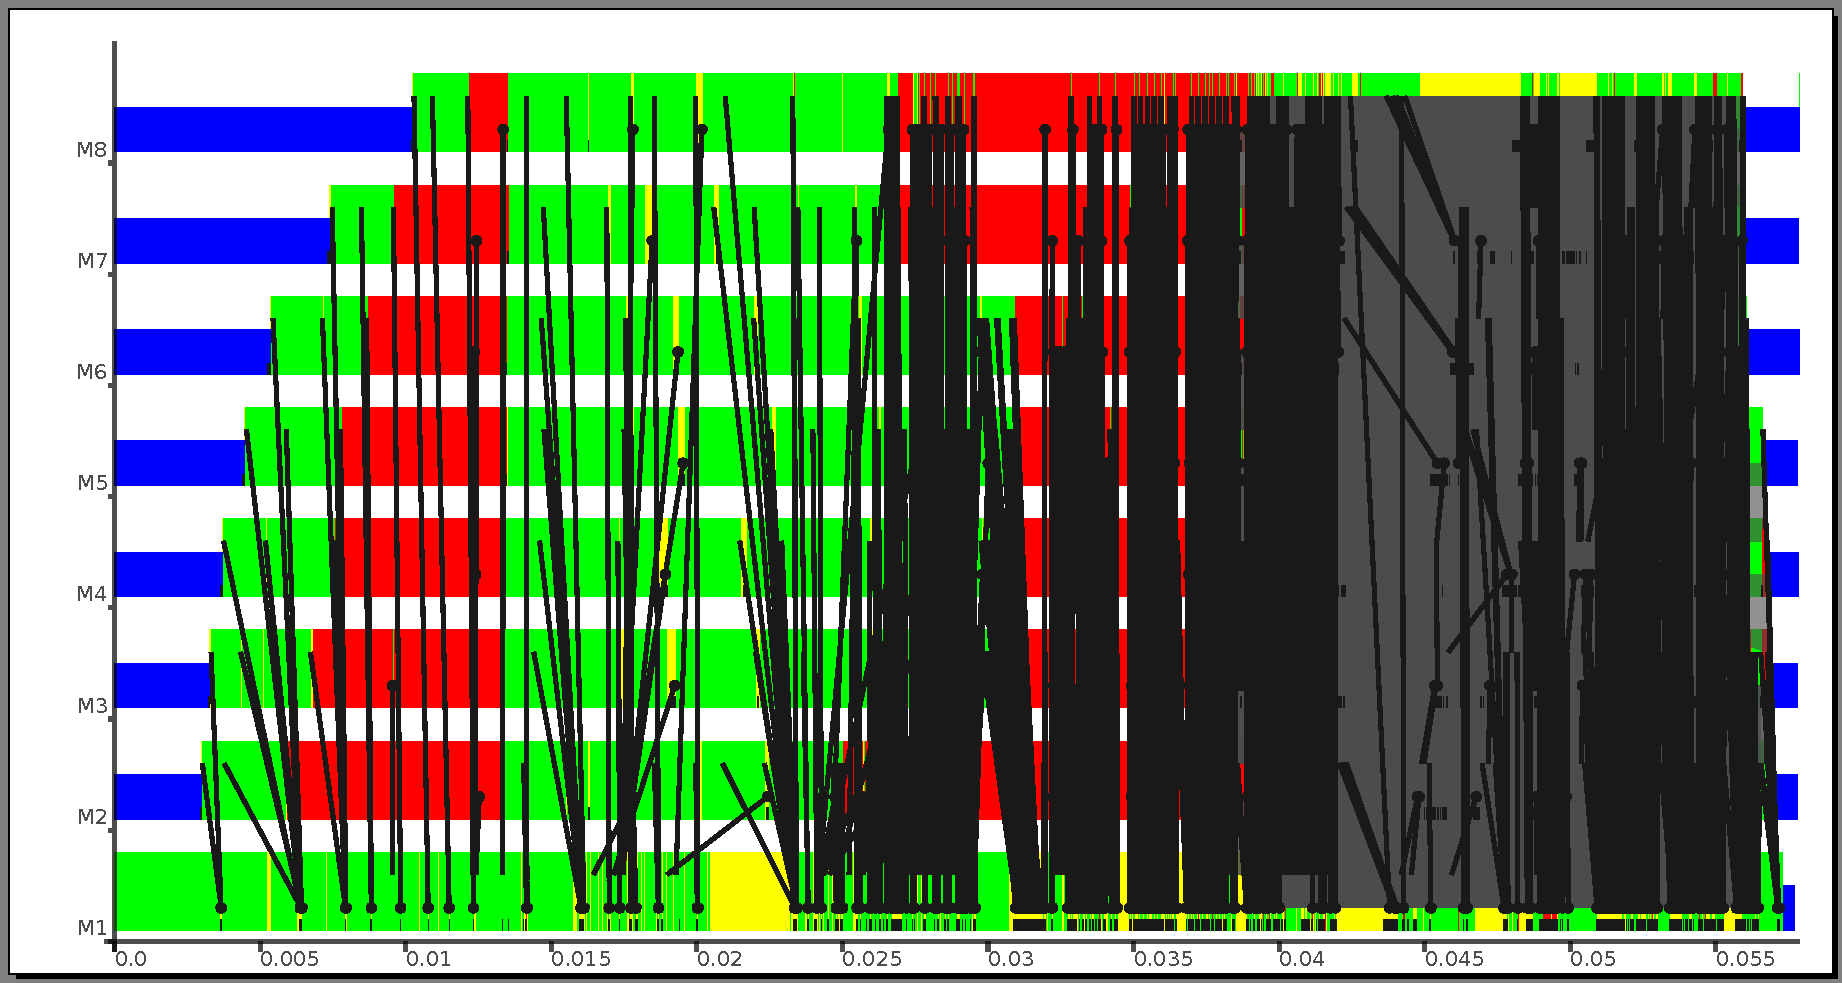
\includegraphics[width=0.9\textwidth]{images/torus_matrix_parrows_scale}
	\caption[without Futures]{Matrix Multiplication with a torus (Parrows)}
\end{figure}

\begin{figure}[ht]
	\centering
	\includegraphics[width=0.9\textwidth]{images/torus_matrix_eden_scale}
	\caption[with Futures]{Matrix Multiplication with a torus (Eden)}
\end{figure}